% 03_methods.tex — Methods / Computational details
% Drafted Session 4ao — block-and-wait review gate.

\section{Methods}\label{sec:methods}

\subsection{Reference-anchored global optimization}\label{sec:methods-search}

We model the amorphous state as the low-energy basin around a chosen
crystalline reference and enumerate that basin with a surrogate-guided
global-optimization search
\cite{gofee2020,gofee2022,agox2022}. The reference is a \emph{physical choice}
the user controls: unique for a host with a single stable phase (here fcc
Pt), a genuine choice for a polymorphic host (Ta, W)
\cite{colin2017,kozhukhovska2026,barmak2017,liubarmak2016,chattaraj2020}.

The search starts from the reference topology. Starting from the
DFT-optimized fcc Pt lattice constant $a = 3.975534$~\AA{} and a $3\times3\times3$
supercell (Pt$_{108}$), we add P interstitials to a target atomic fraction
$C$ via $B = C A / (1 - C)$, giving Pt$_{108}$P$_{27}$ (20~at.\% P) and
Pt$_{108}$P$_{46}$ (30~at.\% P); the undoped Pt$_{108}$ host and a
10~at.\% P system are also considered. Three supercell families are considered,
differing only in the cell expansion applied to the host: $+0\%$
(11.927~\AA), $+3\%$ (12.284~\AA), and $+5\%$ (12.523~\AA); the $+10\%$
family is excluded from scope. Candidate structures are described by the
Oganov--Valle angular fingerprint \cite{oganov2009}, and a Gaussian-process
regression (GPR) surrogate is built from a sum of two radial-basis-function
kernels with a repulsive prior \cite{biswas2017,artrith2018}. A
lower-confidence-bound (LCB) acquisition function ($\kappa = 2$) selects
candidates for density-functional theory (DFT) evaluation \cite{gofee2022}.

Three structure generators enter the candidate mix progressively
\cite{agox2022}, all applying displacements up to 1.5~\AA{}. The
\emph{amorphous randomizer} starts from the reference P-interstitial alloy
and randomly displaces every atom: for each atom it attempts up to 500
random displacements inside a sphere (uniform-volume
sampling), keeping only displacements that stay inside the cell and do not
place the atom too close to a neighbour. This starts the search near the
reference topology. The \emph{rattle generator} displaces a random subset of
atoms, producing small local perturbations of an existing candidate. The
\emph{permutation generator} swaps the positions of atoms of
different species (Pt~$\leftrightarrow$~P) among the interstitial sites, up
to 20 swaps with 20 attempts each, and applies a small rattling displacement
to the swapped atoms, redistributing P among sites to explore different
interstitial arrangements.

\subsection{Iteration timeline}\label{sec:methods-timeline}

The search runs as an iteration counter $i$; the active phase generates $N$
candidates, the surrogate scores them, LCB selects $M$, and DFT evaluates
those $M$ (Fig.~\ref{fig:methods-timeline}). The generator mix and the
relaxation gate switch on at specific iterations. Each system is searched from
multiple independent seeds, each run for 100 iterations.

\begin{figure}[t]
  \centering
  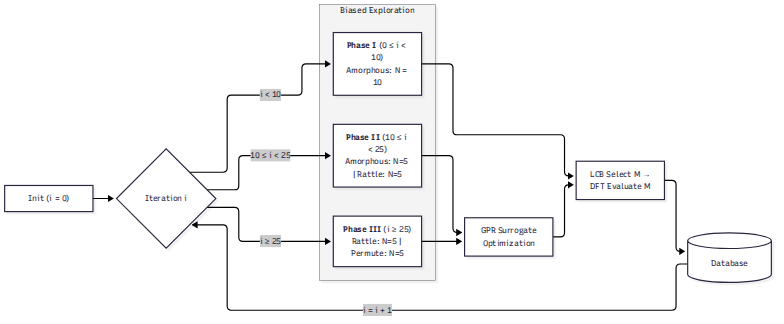
\includegraphics[width=\textwidth]{figures/methods_timeline.png}
  \caption{Iteration timeline of the surrogate-guided search. The search
      runs as an iteration counter $i$; at each iteration the active phase
      generates $N$ candidates, the GPR surrogate scores them,
      the LCB acquisition selects $M$, and DFT evaluates
      those $M$, with the results stored in the database and $i$ incrementing
      by one (feedback loop). The generator mix switches on at specific
      iterations: Phase I ($0 \le i < 10$) uses the amorphous randomizer
      alone; Phase II ($10 \le i < 25$) adds the rattle generator and turns
      on relaxation and LCB guidance; Phase III ($i \ge 25$) swaps in the
      permutation generator.}
  \label{fig:methods-timeline}
\end{figure}

In Phase I ($0 \le i < 10$) the amorphous randomizer alone generates
$N = 10$ candidates. This is the exploration / surrogate-building phase ---
the Gaussian process has no training data yet, so candidates are proposed and
DFT-scored to populate the surrogate (no LCB guidance). In Phase II
($10 \le i < 25$) the rattle generator joins, with $N = 5$ from the amorphous
randomizer plus $N = 5$ from the rattle generator; relaxation begins at
iteration 10 and the search becomes LCB-guided. In Phase III ($25 \le i$) the
permutation generator joins, with $N = 5$ from the rattle generator plus
$N = 5$ from the permutation generator and the amorphous randomizer dropping
out; the search continues under LCB.

Only structures from iteration 10 onward and within 0.1~eV/atom of the
system's global minimum (relative-energy cap, per-system reference) are retained
for analysis.

\subsection{Electronic structure}\label{sec:methods-dft}

Density-functional relaxations are performed with the GPAW code
\cite{gpaw2010,ase2017} using a linear-combination-of-atomic-orbitals (LCAO)
basis (double-zeta-polarized) and the PBE functional, with a single
$\Gamma$-centered $k$-point, Fermi--Dirac smearing of 0.05~eV, and forces
converged to 0.05 eV/\AA{} \cite{madanchi2024}.

\subsection{Crystallinity verification}\label{sec:methods-crystallinity}

Amorphization is quantified by two complementary metrics --- XRD
crystallinity indices and a per-atom Steinhardt bond-orientational order
parameter --- cross-checked against each other \cite{steinhardt1983}.

XRD patterns are simulated with a powder-diffraction calculator (Cu K$\alpha$,
$2\theta$ 10--90$^{\circ}$, Gaussian broadening $\sigma = 0.15^{\circ}$),
reporting peak-fraction and integrated crystallinity indices. Structures are
binned into relative-energy windows (0.1~eV/atom wide, up to 0.5~eV/atom,
relative to the system's global minimum) and a deterministic sample of each
window is averaged \cite{pymatgen2013,ase2017}.

Steinhardt bond-orientational order parameters $q_4$ and $q_6$ are computed
from the first-neighbour shell (cutoff $1.3\times$ the nearest-neighbour
distance); an atom is classified fcc-like when $q_6 > 0.5$ (fcc $q_6 \approx
0.5745$). The crystalline fraction is the mean over the retained ensemble.
Partial radial distribution functions $g_{\mathrm{Pt-P}}(r)$
and $g_{\mathrm{P-P}}(r)$ are computed out to 5.0~\AA{} (200 bins)
\cite{ase2017}.
